\titre{}
\theme{}
\auteur{Nathan Scheinmann}
\niveau{}
\source{}
\type{serie}
\piments{1}
\pts{}
\annee{2526}

\contenu{
  \qrcode{https://coopmaths.fr/alea/?uuid=392b3&id=1mF3-6&n=3&d=10&s=4&cd=1&lang=fr-CH&v=eleve&es=1211001}
	\tcblower
Déterminer l'expression fonctionnelle des deux fonctions ci-dessous à partir des techniques de déplacement de la parabole.
 \begin{center}
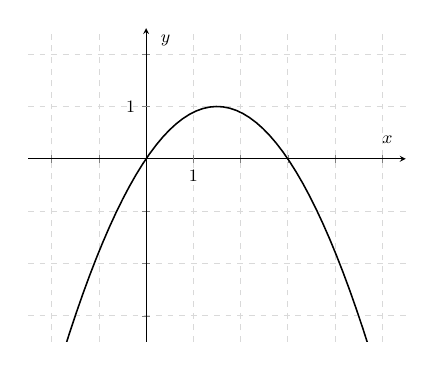
\begin{tikzpicture}[scale=0.7]
  \begin{axis}[
    axis lines=middle,
    xlabel={$x$}, ylabel={$y$},
    every axis x label/.style={at={(ticklabel* cs:0.92)}, anchor=west, yshift=10pt},
    every axis y label/.style={at={(ticklabel* cs:0.92)}, anchor=south, xshift=10pt},
    xmin=-2.5, xmax=5.5,
    ymin=-3.5, ymax=2.5,
    % 1. On définit les positions de la grille pour tous les entiers
    xtick={-2,-1,...,5},
    ytick={-3,-2,...,2},
    % 2. On masque tous les labels par défaut
    xticklabels={},
    yticklabels={},
    % 3. On ajoute spécifiquement le label "1"
    extra x ticks={1},
    extra x tick labels={1},
    extra y ticks={1},
    extra y tick labels={1},
    % Style de la grille
    grid=both,
    grid style={dashed,gray!30},
    tick label style={font=\small},
    xlabel style={font=\small},
    ylabel style={font=\small},
    % On s'assure que les extra ticks ne rajoutent pas de lignes de grille en gras
    extra tick style={grid=none}
  ]
    % f(x) = -1/7x + 11/7
  \addplot[domain=-7:7, samples=100, thick, black]{-4/9*(x-1.5)^2+1};
  \end{axis}
\end{tikzpicture}
\hfill
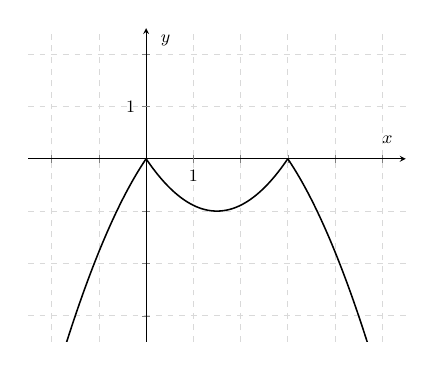
\begin{tikzpicture}[scale=0.7]
  \begin{axis}[
    axis lines=middle,
    xlabel={$x$}, ylabel={$y$},
    every axis x label/.style={at={(ticklabel* cs:0.92)}, anchor=west, yshift=10pt},
    every axis y label/.style={at={(ticklabel* cs:0.92)}, anchor=south, xshift=10pt},
    xmin=-2.5, xmax=5.5,
    ymin=-3.5, ymax=2.5,
    % 1. On définit les positions de la grille pour tous les entiers
    xtick={-2,-1,...,5},
    ytick={-3,-2,...,2},
    % 2. On masque tous les labels par défaut
    xticklabels={},
    yticklabels={},
    % 3. On ajoute spécifiquement le label "1"
    extra x ticks={1},
    extra x tick labels={1},
    extra y ticks={1},
    extra y tick labels={1},
    % Style de la grille
    grid=both,
    grid style={dashed,gray!30},
    tick label style={font=\small},
    xlabel style={font=\small},
    ylabel style={font=\small},
    % On s'assure que les extra ticks ne rajoutent pas de lignes de grille en gras
    extra tick style={grid=none}
  ]
    % f(x) = -1/7x + 11/7
  \addplot[domain=-7:0, samples=100, thick, black]{-4/9*(x-1.5)^2+1};
  \addplot[domain=0:3, samples=100, thick, black]{4/9*(x-1.5)^2-1};
  \addplot[domain=3:7, samples=100, thick, black]{-4/9*(x-1.5)^2+1};
  \end{axis}
\end{tikzpicture}
\end{center}


}
\correction{
	\tcblower

}
